% 2016 年全国卷Ⅱ理科第 5 题：街道最短路径图
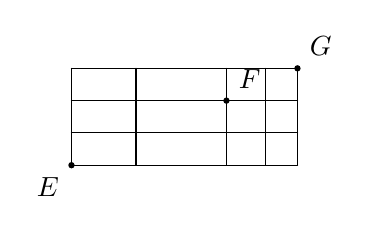
\begin{tikzpicture}[x=0.82cm,y=0.82cm,line cap=round,line join=round]
  % 四列、三行街道网格
  \draw (0,0)--(3.5,0)
        (0,0.5)--(3.5,0.5)
        (0,1.0)--(3.5,1.0)
        (0,1.5)--(3.5,1.5);
  \draw (0,0)--(0,1.5)
        (1.0,0)--(1.0,1.5)
        (2.4,0)--(2.4,1.5)
        (3.0,0)--(3.0,1.5)
        (3.5,0)--(3.5,1.5);
  \fill (0,0) circle (1.15pt);
  \fill (2.4,1.0) circle (1.15pt);
  \fill (3.5,1.5) circle (1.15pt);
  \node[below left=1pt] at (0,0) {$E$};
  \node[above right=1pt] at (2.4,1.0) {$F$};
  \node[above right=1pt] at (3.5,1.5) {$G$};
\end{tikzpicture}
